\documentclass{report}
\usepackage[utf8]{inputenc}
\usepackage[english]{babel}
\usepackage{amsmath}
\usepackage{amsfonts}
\usepackage{amssymb}
\usepackage{amsthm}
\usepackage[basic]{complexity}
\usepackage{tikz}
\usepackage{hyphenat}
\usepackage{graphicx}
\usepackage{mathpazo}
\usepackage{nicefrac}
\usepackage{fontawesome}
\usepackage{multicol}

\usepackage[authoryear]{natbib}

\usepackage{geometry}
\geometry{vmargin = 2.5cm, hmargin = 2.5cm}

\usepackage{array}
\newcolumntype{L}[1]{>{\raggedright\let\newline\\\arraybackslash\hspace{0pt}}m{#1}}
\newcolumntype{C}[1]{>{\centering\let\newline\\\arraybackslash\hspace{0pt}}m{#1}}
\newcolumntype{R}[1]{>{\raggedleft\let\newline\\\arraybackslash\hspace{0pt}}m{#1}}

\renewcommand{\arraystretch}{1.15}

\usepackage{tikz}
\usetikzlibrary{automata, positioning, calc, shapes, arrows, fit}
\newcommand{\circled}[1]{\tikz[baseline=(char.base)]{
		\node[shape=circle, draw, inner sep=0.5pt] (char) {#1};}}

\usepackage[unicode=true, bookmarks=false, breaklinks=true, pdfborder={0 0 1},colorlinks=true]{hyperref}
\hypersetup{linkcolor=blue,citecolor=blue,filecolor=blue,urlcolor=blue}


\begin{document}
	\title{Preflib 2.0}
	\author{Simon Rey}
	\maketitle
	
	\tableofcontents
	
	\chapter{Developing PrefLib}
	
	In this chapter, we detail the inner structure of PrefLib. We will first focus on the folder structure, explaining the role of each file. The second part of this chapter is devoted to the structure of the database. 
	
	The aim of this chapter is to provide all the necessary information to someone who would like to develop further the website. If you are only interested in maintaining the website and do some small changes, the second chapter might be more interesting to you.
	
	\section{Folder Structure}
	
	The folder structure of the project follows that of a typical Django project with one application. The overall Django project is called \texttt{preflib} and the main, and only, django application is called \texttt{preflibApp}. The overall folder structure can be found in Figure \ref{fig:folderStruct}. In what follows, we give an explanation for each folder and files.
	
	\begin{figure}
		\begin{multicols}{2}
			\begin{itemize}
				\item[\faFolderO] preflib
				\begin{itemize}
					\item[\faFileO] settings.py
					\item[\faFileO] urls.py
					\item[\faFileO] wsgi.py
				\end{itemize}
				\item[\faFolderO] preflibApp
				\begin{itemize}
					\item [\faFolderO] management
					\begin{itemize}
						\item[\faFolderO] commands
						\begin{itemize}
							\item[\faFileO] adddataset.py
							\item[\faFileO] generatezip.py
							\item[\faFileO] initializedb.py
							\item[\faFileO] updatemetadata.py
							\item[\faFileO] updatepapers.py
						\end{itemize}
					\end{itemize}
					\item[\faFolderO] preflibtools
					\begin{itemize}
						\item[\faFileO] drawing.py
						\item[\faFileO] graph.py
						\item[\faFileO] instance.py
						\item[\faFileO] properties.py
					\end{itemize}
					\item[\faFolderO] static
					\begin{itemize}
						\item[\faFolderO] adminLogo
						\begin{itemize}
							\item[\faFilesO] images for the admin menu
						\end{itemize}
						\item[\faFolderO] css
						\begin{itemize}
							\item[\faFileO] nouislider.css
							\item[\faFileO] style.css
						\end{itemize}
						\item[\faFolderO] data
						\begin{itemize}
							\item[\faFolderO] CD
							\item[\faFolderO] ED
							\item[\faFolderO] MD
							\item[\faFolderO] types
						\end{itemize}
						\item[\faFolderO] datatoadd
						\item[\faFolderO] js 
						\begin{itemize}
							\item[\faFileO] nouislider.js
						\end{itemize}
						\item[\faFolderO] types
						\begin{itemize}
							\item[\faFileO] dataTypesImages.tex
							\item[\faFilesO] images to present the types
						\end{itemize}
						\item[\faFileO] crisner.png
						\item[\faFileO] gitHubLogo.png
						\item[\faFileO] papers.bib
						\item[\faFileO] preflibADTCite.txt
						\item[\faFileO] preflibADTPaper.pdf
						\item[\faFileO] preflibTrendsComSoCChapter.pdf
						\item[\faFileO] preflibTrendsComSoCCite.txt
					\end{itemize}
					\item[\faFolderO] templates
					\begin{itemize}
						\item[\faFolderO] includes
						\begin{itemize}
							\item[\faFilesO] HTML files that can be included
						\end{itemize}
						\item[\faFolderO] preflib
						\begin{itemize}
							\item[\faFilesO] main HTML files
						\end{itemize}
						\item[\faFileO] 400.html
						\item[\faFileO] 403.html
						\item[\faFileO] 404.html
						\item[\faFileO] 500.html
					\end{itemize}
					\item[\faFolderO] templatetags
					\begin{itemize}
						\item[\faFileO] extratags.py
					\end{itemize}
					\item[\faFileO] admin.py
					\item[\faFileO] apps.py
					\item[\faFileO] choices.py
					\item[\faFileO] forms.py
					\item[\faFileO] models.py
					\item[\faFileO] scripts.py
					\item[\faFileO] urls.py
					\item[\faFileO] views.py
				\end{itemize}
			\end{itemize}
		\end{multicols}
		\caption{Folder Structure of the Project, some less relevant files have been omitted.}
		\label{fig:folderStruct}
	\end{figure}

	\medskip

	We start by detailing the \texttt{preflib} folder.

	\section*{\faFolderO{}  preflib}
	
	The \texttt{preflib} folder contains the files that have an impact on the entire project. This is the highest folder in the Django hierarchy. Files in there are mainly used to set up the global parameters of the project.
	
	\paragraph*{\faFileO{} settings.py} This is the main files for the global settings. Among other things, you will find there the settings for the database, the location of the static files, the debugging mode, the installed applications, ... Not that this file is not on the git for security reasons.
	
	\paragraph*{\faFileO{} urls.py} Use this file to set up the global rules for urls. Whenever a request passed over to Django, this file is used to decide where to send the request next. Handlers for the errors (404, 500, etc...) are also defined there.
	
	\paragraph*{\faFileO{} wsgi.py} This is only used to set up the connection between Django and whatever WSGI tool is used (uWSGI, Gunicorn, Passenger). If you did not understand the previous sentence, you will most likely never have to deal with this file.
	
	\medskip 
	
	Let us now move to the \texttt{preflibApp} folder.
	
	\section*{\faFolderO{} preflibApp}
	
	This folder contains all the files related to the \texttt{preflibApp} Django application. Because this is the only application we have, it thus contains the entire website. Let us first go through the Python files you can find there, sub-folders will be examined afterwards.
	
	\paragraph{\faFileO{} urls.py} This file sets the url patterns for the application. It is in there that the link between an URL and the corresponding view is made. It is also in there that the set of all acceptable URLs (that will not return a 404) is defined. When a request is passed over to Django, the URL is first filtered by the \texttt{urls.py} file in the \texttt{preflib} folder which then calls the url pattern defined in this file to know what view to call for.
	
	\paragraph{\faFileO{} views.py} In Django, a view is a function that takes an input a request and that return a rendered template (an HTML file). This files gathered all the views. This file is probably the most important one as it includes all the code that is run once a request arrives: updating the database, computing so stuff, filter the entries of the database, etc.
	
	\paragraph{\faFileO{} forms.py} Django offers a Python class to deal with forms that makes it easier to check whether they have been properly filled in etc... The forms are defined in this file. It, for instance, includes the search form, the login form, etc.
	
	\paragraph{\faFileO{} models.py} A model in Django is the corresponding Python class to a table in the database. In this files all the models are described in Python. Django then reads through this file and create the database accordingly. The entire database is thus defined in there.
	
	\paragraph{\faFileO{} choices.py} Choices are lists of constant values that are not meant to change often (they would be in the database otherwise). An example is the set of data category for instance. This files gathered them all.
	
	\paragraph{\faFileO{} admin.py} In this file, one can register the models so that they appear in the Django admin website.
	
	\paragraph{\faFileO{} scripts.py} This file defines few useful functions for management purposes.
	
	\paragraph{\faFileO{} apps.py} This is a file that is used by Django to know the application exists. Do not modify it.
	
	\medskip
	
	For the rest of this section, we will explore the sub-folders present in the \texttt{preflibApp} folder.
	
	
	\section*{\faFolderO{} preflibApp/templates}
	
	In Django, a template is an HTML that can incorporate some Django tags in it. They are the main files containing the HTML code of the website. They all are gathered in the \texttt{templates} folder. It contains all the template to render the errors: \texttt{400.html}, \texttt{404.html}, etc. It also contains several sub-folders used to separate the templates based on their use.
	
	\paragraph*{\faFolderO{} includes} This folder gathers all the templates that can be included in some other templates using the \texttt{\{\% include `template' \%\}} Django tag. These files are:
	\begin{itemize}
		\item[\faFileO] footer.html: the footer displayed at the bottom of a page;
		\item[\faFileO] header.html: the header displayed at the top of a page;
		\item[\faFileO] htmlHeaderContent.html: the content of the HTML header that is shared with all pages;
		\item[\faFileO] metadataCategorySearch.html: the code used to render a search widget in the search page;
		\item[\faFileO] paginator.html: the code used to render a paginator in a page.
	\end{itemize}
	
	\paragraph*{\faFolderO{} preflib} This folder gathers the templates used to render all the pages of the website. We list them below.
	\begin{multicols}{2}
		\begin{itemize}
			\item[\faFileO] about.html: the about page
			\item[\faFileO] admin.html: the admin menu
			\item[\faFileO] adminadddataset.html: the admin page for adding datasets
			\item[\faFileO] adminlog.html: the admin page for viewing logs
			\item[\faFileO] adminpaper.html: the admin page for adding a paper
			\item[\faFileO] adminzip.html: the amdin page for zipping the files
			\item[\faFileO] data.html: the data page describing the structure of the data
			\item[\faFileO] dataformat.html: the page explaining the format we use
			\item[\faFileO] datametadata.html: the page describing the metadata
			\item[\faFileO] datapatch.html: the template for rendering a datapatch
			\item[\faFileO] datasearch.html: the search page
			\item[\faFileO] dataset.html: the template for rendering a dataset
			\item[\faFileO] datasetall.html: the template for rendering a category of data
			\item[\faFileO] datatypes.html: the page describing the types
			\item[\faFileO] index.html: the main page of the website
			\item[\faFileO] toolscris.html: the Crisner tool page
			\item[\faFileO] toolsivs.html: the Iterative Voting Simulator page
			\item[\faFileO] toolsskdg.html: the Kidney Dataset Generator page
			\item[\faFileO] userlogin.html: the login page
			\item[\faFileO] usernewaccount.html: the page to create new account
			\item[\faFileO] userprofile.html: the page displaying the profile of a user
		\end{itemize}
	\end{multicols}
	
	\section*{\faFolderO{} preflibApp/templatetags}
	
	The \texttt{templatetags} folder is used to describe user-defined tags that can then be used in the templates. It contains a single file---\texttt{extratags.py}---where the extra tags are defined.
	
	\section*{\faFolderO{} preflibApp/static}
	
	The \texttt{static} folder contains all the static files that are used (unsurprisingly). This folder is the one considered by the \texttt{collecstatic} management command from Django.
	
	\paragraph*{\faFolderO{} adminLogo} This folder gathers all the images of the logo used for the admin menu. Note that it might disappear in some later versions.
	
	\paragraph*{\faFolderO{} css} This folder gathers all the CSS files. There are currently two of them: \texttt{style.css} which is the main CSS file for the style of the website and \texttt{nouislider.css} that is used to render the sliders in the search page.
	
	\paragraph*{\faFolderO{} js} This folder gathers all the JavaScript files. The only file in there is used for the sliders in the search page.
	
	\paragraph*{\faFolderO{} types} This folder gathers the images used to present the types together with the TeX file generating some of them.
	
	\paragraph*{\faFileO{} crisner.png} This image illustrates the Crisner tool.
	
	\paragraph*{\faFileO{} gitHubLogo.png} This image is the GitHub logo displayed in the footer.
	
	\paragraph*{\faFileO{} papers.bib} This bib file is the one read by the management command \texttt{updatepapers}. It contains all the bib entries that are then put in the database as ``papers using PrefLib''.
	
	\paragraph*{\faFilesO{} preflib citations} For the ADT paper and the Trends in ComSoC chapter, the pdf and a txt file with the bib information are provided.
	
	\section*{\faFolderO{} preflibApp/management/commands}
	
	The \texttt{management/commands} folder includes the user-defined commands that one can access using the Django's management tool. Each file in this folder contains a class \texttt{Command} which should contain some specific methods. Importantly, once defined and put in this folder, the command can be accessed as any other management command, for instance from the command line using: \texttt{python3 manage.py adddataset}.
	
	\paragraph*{\faFileO{} adddataset.py} This command is used to add datasets to the database. Only zip files located in the folder \texttt{static/datatoadd} can be retrieved by this command. Two arguments can be passed to the command, either \texttt{--file zipfilename} to add only a specific zip file, or \texttt{--all} to add all the zip files in the \texttt{static/datatoadd} folder to the database.
	
	When adding a dataset, the command unzip the archive in a temporary folder. It then goes through the files to find the info file used to get all the information for the dataset. Then, each file is added to the database, together with its datapatch (if needed). Note that the metadata are not computed when adding a dataset. 
	
	\paragraph*{\faFileO{} generatezip.py} This command is used to generate all the zip files served by the website. It first generates the zip files for the dataset, creating the info file with the entry in the database. In a second time, it generates the zip files per type of data.
	
	\paragraph*{\faFileO{} initializedb.py} This command is only run once, at the very beginning, to populate the database with the entries that are needed. It mainly sets up the metadata.
	
	\paragraph*{\faFileO{} updatemetada.py} This command computes the metadata for the data files. Two options can be passed to the command. When used with \texttt{--dataset datasetAbbreviation}, only the metadata for the given dataset will be computed. One can also use \texttt{--noDrawing} to avoid generating the images for the data file (which takes a lot of time).
	
	For each relevant data file, the command will go through all the \emph{active} metadata (see later what active mean here). Whenever an active metadata applies to the data type of the data file, the corresponding function is called to compute its value. If drawing is allowed, the relevant drawing method is also called.
	
	\paragraph*{\faFileO{} updatepapers.py} This command updates the list of papers that are using Preflib. It reads the bib file \texttt{static/papers.bib} and update the database accordingly.
	
	\section*{\faFolderO{} preflibApp/preflibtools} This folder contains the tools that were developed around PrefLib to work with the data. Note that this version is far from what you can find in the PrefLibTools repository on GitHub. These tools are mainly used to analyze the data when computing the relevant metadata.
	
	\paragraph*{\faFileO{} drawing.py} This file contains all the functions that are used to draw the images representing the data. 
	
	\paragraph*{\faFileO{} graph.py} This file contains the definition of the \texttt{Graph} class that we use to represent graphs and access several useful methods for them.
	
	\paragraph*{\faFileO{} instance.py} This file contains the class used to represent PrefLib instances. The methods for parsing the data file are defined there.
	
	\paragraph*{\faFileO{} properties.py} This file contains a collection of functions used to check whether some properties hold for a given instance. This is the main file used to compute the metadata of the instances.
	
	
	\section{Database Structure}
	
	We now turn to the database used behind the website to organize the datafiles. In igure \ref{fig:database} you will find a complete schematic representation of the database. In what follows, we will give more explanations for each table and row.
	
	\begin{figure}
		\resizebox{\linewidth}{!}{
			\begin{tikzpicture}[shorten > = 5pt, shorten < = 5pt]
				\node[draw, rounded corners = 4pt, thick = 2pt, anchor = north east] (dataset) at (0, 0) {
					\begin{tikzpicture}
						\node[label = above:{\large \textsc{DataSet}}] {\begin{tabular}{rl}
								\textbf{name} & Name of the dataset \\
								\textbf{abbreviation} & Abbreviation of the dataset\\
								\textbf{category} & Extension of the dataset \\
								\textbf{seriesNumber} & Series number of the dataset\\
								\textbf{description} & Few sentences about the dataset \\
								\textbf{requiredCitations} & Papers to cite when using \\& the dataset \\
								\textbf{selectedStudies} & Works related to the dataset \\
								\textbf{publicationDate} & Date at which the dataset \\& has been added \\
								\textbf{modificationDate} & Last time the dataset \\& has been modified
						\end{tabular}};
				\end{tikzpicture}};
				
				\node[draw, rounded corners = 4pt, thick = 2pt, below = 1cm of dataset] (datapatch) {
					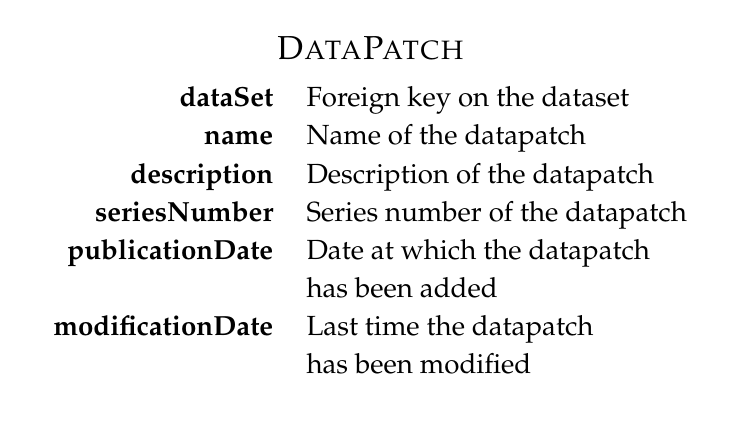
\begin{tikzpicture}
						\node[label = above:{\large \textsc{DataPatch}}] {\begin{tabular}{rl}
								\textbf{dataSet} & Foreign key on the dataset \\
								\textbf{name} & Name of the datapatch \\
								\textbf{description} & Description of the datapatch \\
								\textbf{seriesNumber} & Series number of the datapatch \\
								\textbf{publicationDate} & Date at which the datapatch \\& has been added \\
								\textbf{modificationDate} & Last time the datapatch \\& has been modified
						\end{tabular}};
				\end{tikzpicture}};
				
				\node[draw, rounded corners = 4pt, thick = 2pt, below = 1cm of datapatch] (datafile) {
					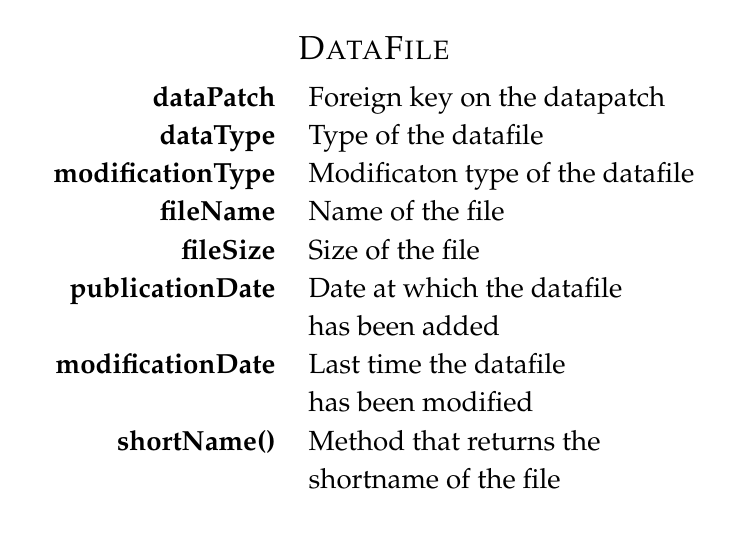
\begin{tikzpicture}
						\node[label = above:{\large \textsc{DataFile}}] {\begin{tabular}{rl}
								\textbf{dataPatch} & Foreign key on the datapatch \\
								\textbf{dataType} & Type of the datafile\\
								\textbf{modificationType} & Modificaton type of the datafile\\
								\textbf{fileName} & Name of the file  \\
								\textbf{fileSize} & Size of the file \\
								\textbf{publicationDate} & Date at which the datafile \\& has been added \\
								\textbf{modificationDate} & Last time the datafile \\& has been modified \\
								\textbf{shortName()} & Method that returns the \\& shortname of the file
						\end{tabular}};
				\end{tikzpicture}};
				
				\node[draw, rounded corners = 4pt, thick = 2pt, anchor = north west] (metadata) at (1, 0) {
					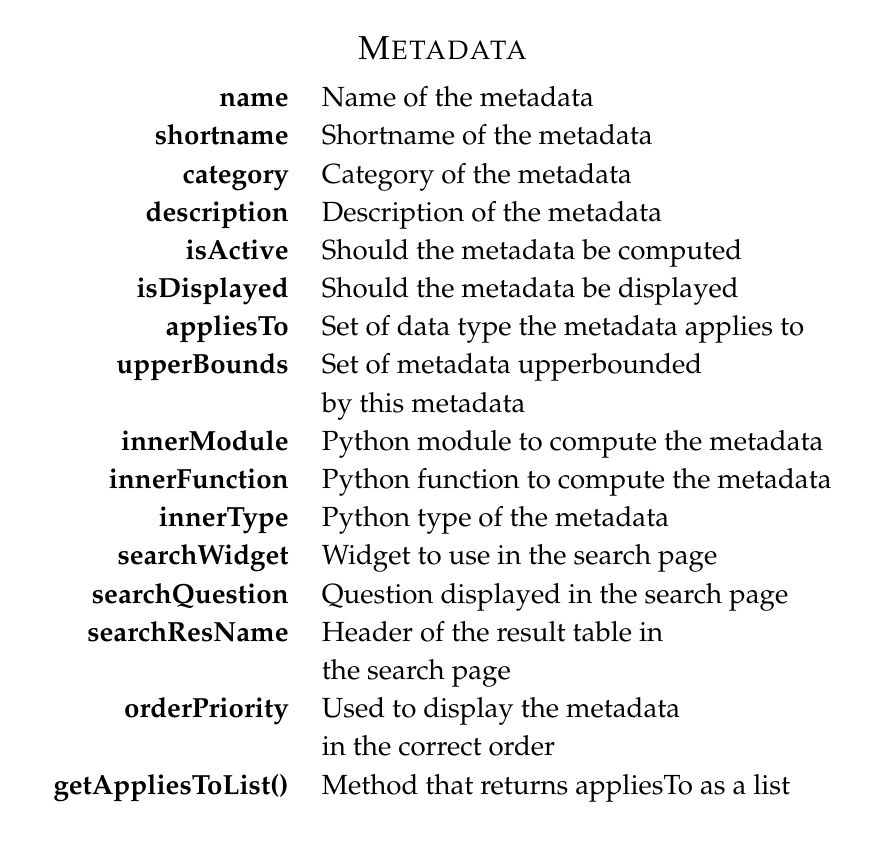
\begin{tikzpicture}
						\node[label = above:{\large \textsc{Metadata}}] {\begin{tabular}{rl}
								\textbf{name} & Name of the metadata \\
								\textbf{shortname} & Shortname of the metadata \\
								\textbf{category} & Category of the metadata \\
								\textbf{description} & Description of the metadata \\
								\textbf{isActive} & Should the metadata be computed \\
								\textbf{isDisplayed} & Should the metadata be displayed \\
								\textbf{appliesTo} & Set of data type the metadata applies to \\
								\textbf{upperBounds} & Set of metadata upperbounded \\& by this metadata\\
								\textbf{innerModule} & Python module to compute the metadata \\
								\textbf{innerFunction} &  Python function to compute the metadata \\
								\textbf{innerType} & Python type of the metadata \\
								\textbf{searchWidget} & Widget to use in the search page\\
								\textbf{searchQuestion} & Question displayed in the search page\\
								\textbf{searchResName} & Header of the result table in \\& the search page\\
								\textbf{orderPriority} & Used to display the metadata \\& in the correct order\\
								\textbf{getAppliesToList()} & Method that returns appliesTo as a list
						\end{tabular}};
				\end{tikzpicture}};
				
				\node[draw, rounded corners = 4pt, thick = 2pt, below = 1cm of metadata] (dataprop) {
					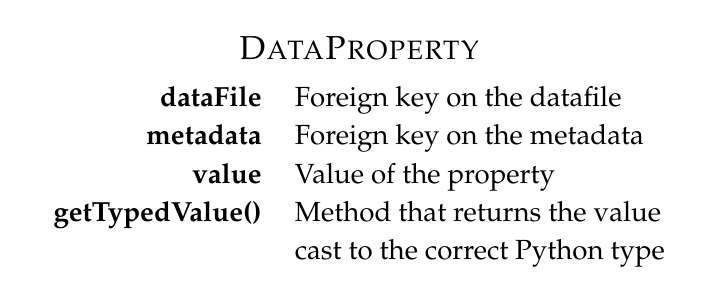
\begin{tikzpicture}
						\node[label = above:{\large \textsc{DataProperty}}] {\begin{tabular}{rl}
								\textbf{dataFile} & Foreign key on the datafile \\
								\textbf{metadata} & Foreign key on the metadata \\
								\textbf{value} & Value of the property \\
								\textbf{getTypedValue()} & Method that returns the value \\& cast to the correct Python type 
						\end{tabular}};
				\end{tikzpicture}};
				
				\draw[->] (dataset) edge (datapatch);
				\draw[->] (datapatch) edge (datafile);
				\draw[->] (metadata) edge (dataprop);
				\draw[->] (dataprop) edge (datafile);
				
				\node[draw, rounded corners = 4pt, thick = 2pt, below = 1cm of datafile] (paper) {
					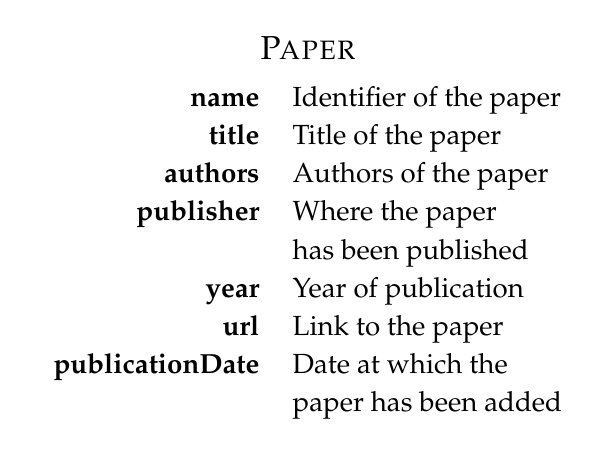
\begin{tikzpicture}
						\node[label = above:{\large \textsc{Paper}}] {\begin{tabular}{rl}
								\textbf{name} & Identifier of the paper \\
								\textbf{title} & Title of the paper \\
								\textbf{authors} & Authors of the paper \\
								\textbf{publisher} & Where the paper \\& has been published \\
								\textbf{year} & Year of publication \\
								\textbf{url} &  Link to the paper \\
								\textbf{publicationDate} & Date at which the \\& paper has been added
						\end{tabular}};
				\end{tikzpicture}};
				
				\node[draw, rounded corners = 4pt, thick = 2pt, below = 1cm of dataprop] (user) {
					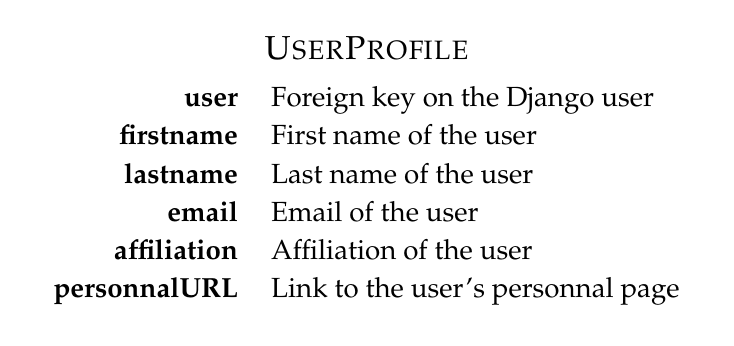
\begin{tikzpicture}
						\node[label = above:{\large \textsc{UserProfile}}] {\begin{tabular}{rl}
								\textbf{user} & Foreign key on the Django user \\
								\textbf{firstname} & First name of the user \\
								\textbf{lastname} & Last name of the user \\
								\textbf{email} & Email of the user \\
								\textbf{affiliation} & Affiliation of the user \\
								\textbf{personnalURL} &  Link to the user's personnal page
						\end{tabular}};
				\end{tikzpicture}};
				
				\node[draw, rounded corners = 4pt, thick = 2pt, below = 1cm of user] (log) {
					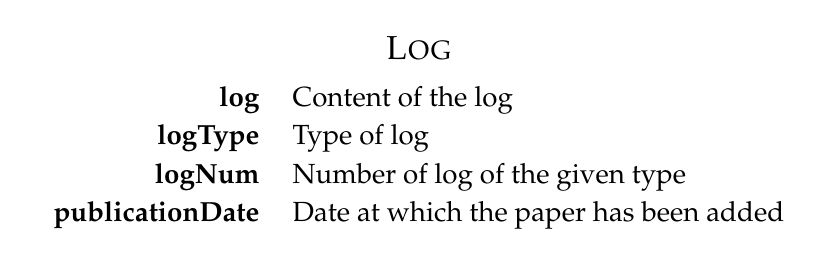
\begin{tikzpicture}
						\node[label = above:{\large \textsc{Log}}] {\begin{tabular}{rl}
								\textbf{log} & Content of the log \\
								\textbf{logType} & Type of log \\
								\textbf{logNum} & Number of log of the given type \\
								\textbf{publicationDate} & Date at which the paper has been added
						\end{tabular}};
				\end{tikzpicture}};
		\end{tikzpicture}}
		\caption{Structure of the database}
		\label{fig:database}
	\end{figure}
	
	\subsection*{\faDatabase{} \textsc{DataFile}}
	
	The most fundamental entity for Preflib is the datafile. The \textsc{DataFile} table contains a reference to all the datafiles that are in Preflib. The table does not contain the data in itself---it is stored in a file and not in the database---but all the relevant information about it: some basic details and datapatch in which the file is.
	
	In what follows, we provide more details on each of the columns of this table:
	\begin{itemize}
		\item \textbf{dataPatch}: this is a foreign key on a datapatch entry. It indicates the datapatch in which the datafile is.
		\item \textbf{dataType}: the type of the datafile, it should be one of soc, soi, toc, toi, tog, mjg, wmg, pwg, wmd, dat, csv. This field is linked to the \texttt{DATATYPES} choice list to get a consistent database.
		\item \textbf{modificationType}: the modification type of the datafile, it should be one of original, induced, imbued, synthetic. This is linked to the \texttt{MODIFICATIONTYPES} choice list to get a consistent database.
		\item \textbf{fileName}: the name of the file containing the actual data.
		\item \textbf{fileSize}: the size of the file containing the actual data.
		\item \textbf{publicationDate}: the date at which the file has been added to the database.
		\item \textbf{modificationDate}: the date at which the file has been last modified.
	\end{itemize}
	
	The Python class also introduces a method called \texttt{shortName()} which can be used to get the shortname of a datafile. This method is used for the name of the datafiles in the result table of the search page. Note that this is a method of the Python class and not a column of the table in the database.
	
	\subsection*{\faDatabase{} \textsc{DataPatch}}
	
	The datapatch is the first level of classification of the datafile. It contains several datafile of different datatype. All the datafiles are based on the same preferences but the representation, the datatype, is different.
	
	In what follows, we provide more details on each of the columns of this table:
	\begin{itemize}
		\item \textbf{dataSet}: this is a foreign key on a dataset entry. It indicates the dataset in which the datapatch is.
		\item \textbf{name}: the name of the datapatch.
		\item \textbf{description}: a short description of the datapatch. It usually indicates the exact content of the patch with respect to the full dataset. For instance in the Irish elections dataset, it could be ``Dublin 2006''.
		\item \textbf{seriesNumber}: the identifier of the datapatch, this is a 8 digits number.
		\item \textbf{publicationDate}: the date at which the datapatch has been added to the database.
		\item \textbf{modificationDate}: the date at which the datapatch has been last modified.
	\end{itemize}
	
	\subsection*{\faDatabase{} \textsc{DataSet}}
	
	A dataset is a collection of datapatches. The datapatches will typically represent different years of the same election, all gathered in a unique dataset.
	
	In what follows, we provide more details on each of the columns of this table:
	\begin{itemize}
		\item \textbf{name}: the name of the dataset
		\item \textbf{abbreviation}: the abbreviation of the dataset. That will be the name of the zip archive containing the dataset for instance.
		\item \textbf{category}: the category of the dataset, it should be one of ED, MD, CD. This field is linked to the \texttt{DATACATEGORY} choice list to get a consistent database.
		\item \textbf{seriesNumber}: the identifier of the dataset, this is a five digit number.
		\item \textbf{description}: a brief description of the dataset, usually a paragraph. It is rendered as HTML code so any HTML tags can be used there.
		\item \textbf{requiredCitations}: a list of papers that are to be cited if this dataset is used in a publication.
		\item \textbf{selectedStudies}: a set of papers that are relevant for this dataset, typically showing examples of what have been done with it.
		\item \textbf{publicationDate}: the date at which the dataset has been added to the database.
		\item \textbf{modificationDate}: the date at which the dataset has been last modified.
	\end{itemize}
	
	\subsection*{\faDatabase{} \textsc{DataProperty}}
	
	A dataproperty is an additional information about a given datafile. It can have to do about the general properties of the data (number of candidates...) or about some more specific structure of the data (single-peakedness...).
	
	In what follows, we provide more details on each of the columns of this table:
	\begin{itemize}
		\item \textbf{dataFile}: a foreign key on a datafile entry. It indicates the datafile the dataproperty is about.
		\item \textbf{metadata}: a foreign key on a metadata entry. It indicates the type of metadata the dataproperty is about.
		\item \textbf{value}: the actual value of the metadata for the given datafile. It can be of many types, most likely it will be either a number or a boolean.
	\end{itemize}

	The Python class also introduces the method \texttt{getTypedValue()} which returns the value of the dataproperty but cast in the correct Python type (it is otherwise a string). This method is mainly used to filter the datafiles in the search tool. Note that this is a method of the Python class and not a column of the table in the database.
	
	\subsection*{\faDatabase{} \textsc{Metadata}}
	
	A metadata is a type of information about a datafile. The actual value of the datafile for a given metadata is stored in \textsc{DataProperty} table.
	
	In what follows, we provide more details on each of the columns of this table:
	\begin{itemize}
		\item \textbf{name}: the name of the metadata
		\item \textbf{shortname}: the shortname of the metadata, it should not contain any space character. It is used in the internal of the search tool.
		\item \textbf{category}: the category of the metadata, it should be one of general, preference, ballot. This filed is linked to the \texttt{METADATACATEGORIES} choice list to get a consistent database.
		\item \textbf{description}: the description of the metadata as displayed in the metadata page.
		\item \textbf{isActive}: a boolean value indicating whether the metadata should be considered when computing the dataproperties through the \texttt{updatemetadata} management command.
		\item \textbf{isDisplayed}: a boolean value indicating whether the metadata should be displayed in the website. Some metadata can be interesting for sanity checks but not as a search field for instance.
		\item \textbf{appliesTo}: a string representing all the type of data the metadata applies to. The types should be separated by a coma ``,'' and without spaces, e.g., ``toi,toc,soi,toc''
		\item \textbf{upperBounds}: a many-to-many relationship on metadata entries. Any metadata in the many-to-many set is upper-bounded by the current metadata. It of course only applies to metadata with numeric values. It is used in the search page to synchronize the sliders of some metadata.
		\item \textbf{innerModule}: the internal Python module used to compute the value of the metadata. This is how the \texttt{updatemetadata} command knows in which module the function to call to create a dataproperty entry is.
		\item \textbf{innerFunction}: the internal Python function used to compute the value of the metadata. This is how the \texttt{updatemetadata} command knows which function to call to create a dataproperty entry.
		\item \textbf{innerType}: the internal Python type of the metadata. That type is used to cast the value correctly when using the \texttt{getTypedValue()} method of a dataproperty object.
		\item \textbf{searchWidget}: the widget used to display the corresponding field in the search page form. It should be one of ternary, range. This filed is linked to the \texttt{SEARCHWIDGETS} choice list to get a consistent database.
		\item \textbf{searchQuestion}: the question displayed together with the widget on the search page.
		\item \textbf{searchResName}: the header of the corresponding column used in the result table of the search page.
		\item \textbf{orderPriority}: a integer value that is used to order the metadata in a fixed way. This is used to fix the order of the metadata page for instance. 
	\end{itemize}

	The Python class also defined the \texttt{getAppliesToList()} method which returns the appliesTo field but as a list of string instead of just one full string. Note that this is a method of the Python class and not a column of the table in the database.

	\subsection*{\faDatabase{} \textsc{Paper}}
	
	This table stores the information about the papers that are using Preflib displayed on the front page.
	
	In what follows, we provide more details on each of the columns of this table:
	\begin{itemize}
		\item \textbf{name}: identifier of the paper, typically the bib identifier in the bib file.
		\item \textbf{title}: the title of the paper.
		\item \textbf{authors}: the authors of the paper, just the initial of the first name, without a dot, and the family name afterwards.
		\item \textbf{publisher}: the conference, journal, venue... in which the paper has bee published.
		\item \textbf{year}: the year of publication of the paper.
		\item \textbf{url}: a URL linking the to paper.
		\item \textbf{publicationDate}: the data at which the paper has been added to the database.
	\end{itemize}

	\subsection*{\faDatabase{} \textsc{UserProfile}}
	
	All the information about the users that are not in the Django User class are present in this table. Note that for the moment this is not used.
	
	In what follows, we provide more details on each of the columns of this table:
	\begin{itemize}
		\item \textbf{user}: a foreign key on the Django user entry.
		\item \textbf{firstname}: the first name of the user.
		\item \textbf{lastname}: the last name the user.
		\item \textbf{email}: the email of the user.
		\item \textbf{affiliation}: the affiliation of the user.
		\item \textbf{personnalURL}: a URL linking to the website of the user.
	\end{itemize}
	
	\subsection*{\faDatabase{} \textsc{Log}}
	
	Logs of what is happening in the inside are gathers in this table.
	
	In what follows, we provide more details on each of the columns of this table:
	\begin{itemize}
		\item \textbf{log}: the actual content of the log. It is rendered as HTML code so any tag in there will be rendered accordingly.
		\item \textbf{logType}: the type of the log.
		\item \textbf{logNum}: the identifier of the log inside its category of log.
		\item \textbf{publicationDate}: the data at which the log has been added to the database.
	\end{itemize}


	\chapter{Maintaining PrefLib}
	
\end{document}